

\chapter*{Preface}

The summer of 2013 was very good; we found a series of papers published by Gregory D. Smith and his coauthors. We spent several weeks trying to understand the paper \cite{Huertas2007}, which introduces and carefully studies a stochastic model of calcium release from internal stores in cells. Then we found a whole series of papers \cite{Mazzag2005,Williams2007,Williams2008,Huertas2010} and the results more or less kept us busy for months. The beauty of the theory presented in these papers is that they introduce a systematic way of analyzing models that are of great importance for understanding essential physiological processes.

\bigskip

So what is this theory about? It has been fairly well known for a while that stochastic models are useful in studying the release of calcium ions from internal storage in living cells. Some authors even argue that this process {\it is} stochastic. That is debatable, but it is quite clear that stochastic models are well suited to study such processes. Stochastic models are also very well suited to study the change of the transmembrane potential resulting from the flow of ions through channels in the cell membrane. Both these processes are of fundamental importance in understanding the function of excitable cells. In both applications, ions flow from one domain to another according to electrochemical gradients, depending on whether the channel is in a conducting or non-conducting mode. The state of the channel is described by a Markov model, which is a wonderful tool used to systematically represent how an ion channel or a receptor opens or closes based on the surrounding conditions. In this context, the contribution of the papers listed above is to present a systematic way of analyzing the stochastic models in terms of formulating deterministic differential equations describing the probability density distributions of the states of the Markov models.
\bigskip

As pointed out in the papers by Smith et al., this approach is not really new; the authors cite a number of earlier papers and we have been quite influenced by the paper of Nykamp and Tranchina \cite{Nykamp2000} because of its elegant way of developing the deterministic differential equation describing the probability density functions of the states involved in the stochastic process.
The key observation is that we can study stochastic release in two fundamentally different ways: 1) We can run a number of simulations using a stochastic model. Because of the stochastic state of the channel, the results will differ, but we can gather numerous results and summarize them in terms of histograms describing the probability density functions of being in a given state. 2) We can find a deterministic partial differential equation modeling the probability density functions and obtain the distributions by solving this system numerically. By increasing the number of simulations in 1) and by refining the numerical discretization in 1) and 2), we observe that the results of the two methods converge to the same distributions. Therefore, we have a very powerful tool for analyzing the stochastic models: We can simply solve deterministic partial differential equations to find the probability density functions. In some simple cases the deterministic partial differential equations can be studied analytically and no numerical solution is needed.  The relation between the stochastic simulation and the solution
of the deterministic partial differential equations will be studied repeatedly in these notes.


\bigskip
More recently we found the book by Bressloff \cite{Bressloff2014} to be an astonishing source of material concerning stochastic processes in cells. It will clearly become a standard reference in the field together with its companion volume \cite{Bressloff2014w}. The theory of stochastic processes is also introduced in a most readable manner by Jacobs \cite{Jacobs2010} and elements of the theory are covered in the monumental work of Keener and Sneyd \cite{Keener2010_I,Keener2010_II}.


\bigskip

One reason for our enthusiasm in finding the papers listed above is that, for a while, we have been trying to understand how to theoretically devise suitable drugs for mutations affecting both ion channels and receptors. It has been clear for some time that the effect of mutations on ion channels and various receptors can be successfully modeled using Markov models to describe the state of the channel. A comprehensive review is presented by Rudy \cite{Rudy2012} (see also Rudy and Silva \cite{Rudy2006}). Clancy and Rudy and their co-authors (e.g., \cite{Clancy2007}) have also shown how to use Markov models to describe the function of various drugs aimed at repairing the function of mutated channels or receptors. This is very useful, since it allows simulation based on stochastic models and the models can also be interpreted as continuous representations for whole cell simulations. However, analysis of the Markov models is taken to a new level by the introduction of probability density functions defined in terms of deterministic partial differential equations.

\bigskip

Our approach has been as follows: Let the properties of the drug be free parameters and use a setup based on Markov models to find the best possible drugs. This problem is much easier to approach using the results of Smith et al. because it amounts to understanding how the solution of the extended system of partial differential equations (including the effect of the drug)  behaves as a function of the parameters characterizing the drug. Typically, we will end up comparing the solutions of three systems of partial differential equations: 1) a system modeling the dynamics of healthy (wild type) cells, 2) a system modeling the dynamics of non-healthy (mutant) cells, and 3) a system modeling the dynamics of non-healthy cells with a drug added to repair the effect of the mutation. {\it The problem we would like to address is how to adjust the parameters describing the drug such that the solution of 3) is as close to the solution of 1) as possible.} This turns out to be much easier using a deterministic system of partial differential equations describing the probability density functions than using stochastic simulations.

\bigskip

 We have decided to present our results in the form of lecture notes. There are several reasons for this choice. First, we strongly believe that the theory described above is very useful and we want to help make it as comprehensible as possible. That is more or less impossible to do in scientific papers because their focus must be on new results and not on careful derivations of established insights. A second reason is that the problem of understanding cell physiology and how drugs affect their function is inherently multidisciplinary and we therefore write these notes in such a way that we hope readers who are not primarily applied mathematicians can understand.  We also hope to give applied mathematicians glimpses of interesting problems of great importance.
\bigskip

As mentioned above, these notes aim to explain known theory that we think can be useful to researchers working on a mathematical understanding of living cells.  There are also new results. We show in some detail how to derive formulas describing the optimal properties of theoretical drugs. Most of the results are stated for rather simple models, but it is quite clear that the methods can be extended to more intricate cases.
\bigskip

The million dollar question when you read these notes is, of course, can these drugs actually be created? Do they exist? We do not know. We know that Markov models have been used to successfully represent the actions of drugs, but is it possible go the other way and first compute what properties the drug should have and then create it?  We have found no clear answers in the literature or through discussions with colleagues, so we decided to just formulate these ideas as precisely as possible in the hopes that someone will find them useful. We have tried to carefully underline in the notes that we are discussing {\it theoretical drugs} and we state in many places that this work is about possible drugs.

\bigskip
\bigskip

{\bf Acknowledgments}

\bigskip

It is pleasure to thank Dr Martin Peters at Springer for a very fruitful collaboration through many years.

We would also like to thank the six reviewers of these notes. One reviewer wrote an unusually comprehensive and encouraging report counting seven pages; we spent two months working on his or her comments and it was clearly worth the effort. We have never experienced a referee report of equal depth and usefulness and we deeply appreciate the reviewer's labor.

These lecture notes were largely written during visits to the University of California, San Diego, and the authors are grateful for the hospitality of the Department of Bioengineering and the Department of Computer Science and Engineering.

Finally, we would like to thank Karoline Horgmo J\ae ger, who read the entire document twice and found numerous small (and actually some not so small) errors. Her efforts are highly appreciated. We would also like to thank Achim Schroll for helpful discussions regarding the hyperbolic problems encountered in this text.

This work was supported by a Centre of Excellence grant from the Norwegian Research Council to the Center for Biomedical Computing at Simula Research Laboratory.

\bigskip
\bigskip

Simula Research Laboratory, October 2015,

\bigskip


Aslak Tveito and Glenn T. Lines

\bigskip
\bigskip

Corresponding author: aslak@simula.no



\chapter{Background: Problem and methods}
\label{Background}

Drugs are generally devised to alter the function of cells in a favorable manner. The actions of drugs can in some cases be represented by mathematical models often phrased in terms of differential equations. Our aim in these notes is to study such models and show how the effect of drugs can be optimized. More precisely, drugs are represented in terms of a set of parameters and we show how optimal drugs can be characterized by tuning the parameters. Our approach is to consider models of a healthy cell and a non-healthy cell and a model of a non-healthy cell to which a drug has been applied. The problem we are trying to resolve is how to tweak the parameters of the drug such that the drugged non-healthy cell behaves as similarly to the healthy cell as possible.

We will use this approach to address two processes of immense importance in physiology:
1) voltage-gated ion channels and 2) calcium release from storage structures inside the cell. We will also study combinations of these processes occurring in a space in which the release through voltage-gated ion channels interacts with calcium release from the internal storage structures.

Both processes can be affected by disease and by mutations. In these notes we will concentrate on wild type (healthy) cells and mutant cells. We will assume that the behavior of the wild type cell can be described in terms of Markov models  and that a Markov model can represent the effects of the mutation.

\section{Action potentials}

Suppose a group of engineers were given the task of developing a pump weighing about 300 g that is supposed to work uninterruptedly and basically without maintenance for about 80 years, pump about 7000 liters of blood every day, and beat every second. The group would---and should---agree that the task is impossible but, under pressure from their employer, they would probably agree that the mechanism would have to be extremely simple. Fortunately for us all, the pump has already been developed by evolution, but it is very far from being simple; it is an extremely complex piece of machinery, so complex that how it works  is still not completely understood. For an intriguing illustration of this, the reader is encouraged to consult the fascinating joint paper by Lakatta and DiFrancesco \cite{Lakatta2009} in which they debate the following fundamental question: How is the heartbeat initiated? It is remarkable that such a basic question is still open. Two plausible and completely different mechanisms are discussed, with supporting experimental data and mathematical models for both. The interested reader can also consult Li et al. \cite{Li2013} for an introduction to this discussion.

Even if the exact mechanism for initiating the heartbeat is still under debate, it is completely clear that every normal heartbeat is initiated in the sinoatrial node. From that node, an electrochemical wave spreads throughout the cardiac muscle. With every beat, billions of cardiac cells undergo an action potential that is a characteristic temporal change of the transmembrane potential of the cell $V$, defined by
\[ V = V_i-V_e, \]
where $V_i$ and $V_e$ are the intracellular and extracellular electrical potentials, respectively.

%A typical action potential is given in Figure \ref{Introduction_L:grandi} computed using the model of ventricular cardiac cells developed by Grandi et al. \cite{Grandi2010B}.
In Figure \ref{Introduction_L:AP_Jost2009}  we show an action potential obtained by measurements. The recordings are taken from the paper by Jost et al. \cite{Jost2009}. Mathematical models have been used to represent action potentials ever since the groundbreaking paper by Hodgkin and Huxley \cite{Hodgkin1952} from 1952. The first models of cardiac cells were developed by Noble \cite{Noble1960,Noble1962} in 1960--62. In Figure \ref{Introduction_L:grandi} an action potential is presented based on the mathematical model of ventricular cardiac cells developed by Grandi et al. \cite{Grandi2010B}.

FIGURE: [fig/Introduction_L_AP_Jost2009.png, width=500 frac=0.8]  Action potentials obtained by measurements taken from Jost et al. \cite{Jost2009}. label{Introduction_L:AP_Jost2009}

FIGURE: [fig/Introduction_L_grandi.pdf, width=500 frac=0.8] Action potential computed using the model of Grandi et al. \cite{Grandi2010B}.  label{Introduction_L:grandi}

When an electrical wave of the increased transmembrane potential approaches a cell, the cell's transmembrane potential is elevated above a critical value. This elevation leads to the opening of sodium channels, resulting in a huge influx of sodium ions into the cell. This rapid process dramatically increases the transmembrane potential and is referred to as the upstroke of the action potential.

When the transmembrane potential increases, voltage-gated calcium channels in the cell membrane open and calcium ions flow into the cell because of the huge difference in concentrations; the extracellular concentration of calcium ions is much greater than the intracellular (cytosolic) concentration when the cell is at rest. The increased concentration of calcium ions within the cell triggers the opening of channels to internal stores and a great deal more calcium floods into the cytosol.  The increased level of calcium in the cytosol leads to the cell's contraction, which is basically the main goal of the whole operation. Then everything returns to the resting state: Calcium is pumped out of the cell and into internal stores---every cell prepares for a new wave.

Even if this process is amazingly stable and versatile and a masterpiece by any standard in the universe, it is not infallible. It can be harmed by disease, by  the side effects of drugs, and by mutations. In these lecture notes, we shall focus on the effect of mutations and search for theoretical drugs that can, in principle, repair the effect of dangerous mutations. The study of mutations affecting cardiac cells is a huge field and we will simply look at prototypical models that capture the characteristic effects of well-known mutations. Our main objective is to present methods for computing characterizations of optimal theoretical drugs using prototypical models of ion release.

Most of these lecture notes will be focused on what happens in single ion channels. However, in the final chapter we will return to the
action potential of the whole cell.

\section{Markov models}
\label{markovintro}

The cell membrane is densely populated with ion channels that can open and close to control the flow of ions across the cell membrane. In Figure
\ref{Introduction:na_cropped}, we show the recordings of a single channel and we note the frequent transitions between the open and closed states and how the frequency changes with the transmembrane potential. It is commonly believed that the state of a single channel is adequately modeled using a stochastic approach. Actually, it is common to claim that the process is stochastic. It is hard,  if not impossible, to prove that something is stochastic, but for modeling purposes it suffices to state that a stochastic approach leads to reasonable models of the gating dynamics.



\begin{figure}[h]\centering
\hbox{
%\includegraphics[width=0.8\linewidth]{Introduction/na_cropped.png}
%\includegraphics[width=0.2\linewidth]{Introduction/scales.png}
%\includegraphics[width=0.15\linewidth]{Introduction/shaya_scales.png}
%\includegraphics[width=0.8\linewidth]{Introduction/shaya20_60.png}
\includegraphics[scale=0.4]{Introduction_L/shaya_scales.png}
\includegraphics[scale=0.4]{Introduction_L/shaya20_60.png}
}
\caption{Single-channel recording of a sodium current (from Shaya et al \cite{Shaya2011}).
The levels of the current indicate whether the channel is closed (as indicated in the figure) or open. The probability that the channel is open is low at -60 mV, higher at -40 mV, and even higher at -20mV. \label{Introduction:na_cropped}}
\end{figure}



A Markov model in its simplest form is usually written as the chemical reaction scheme
\begin{equation}
C\underset{k_{co}}{\overset{k_{oc}}{\leftrightarrows}}O, \label{Markov1}
\end{equation}
where $k_{oc}$ and $k_{co}$ are reaction rates that may depend on the transmembrane potential. We will return to the interpretation of this notation many times, but let us just roughly describe what it means. Suppose at a given time $t$ that the gate is open so the channel is in state $O$ and suppose that $\Delta t$ is a very short time \GTLV[step]{interval}. Then (\ref{Markov1}) states that the probability that the channel changes state from open to closed is given by $ k_{oc} \Delta t$. Similarly, if the channel is closed (C), the probability for a change to the open state is given by $ k_{co} \Delta t$.

More formally, we let $S=S(t)$ denote a random variable representing
the state of the channel at time $t,$ so $S\in\left\{  O,C\right\}  $. Then
the transition rates $k_{oc}$ and $k_{co}$ give the probability of changing
state during a small time interval $\Delta t:$
\[
k_{oc}\Delta t=\text{Prob}\left[  S(t+\Delta t)=C\mid S(t)=O(t)\right]
\]
and
\[
k_{co}\Delta t=\text{Prob}\left[  S(t+\Delta t)=O\mid S(t)=C(t)\right],
\]
respectively. With this notation, we easily see that we can play with the properties of the channels by changing the values of the parameters $ k_{oc}$ and  $k_{oc}$. We also see that we can make the reaction scheme dependent on the transmembrane potential $V$  (mV) by allowing the reaction terms to depend on $V.$


The case of just one closed and one open state is particularly simple but it is still the base model and it is frequently used in modeling ion channels.
However, much more intricate models have been derived and one is shown in Figure \ref{clancy}. It represents a Markov model with one open state, three closed states, and five inactivated\footnote{Inactivated states are discussed in Chapter \ref{inactivated}.  } states.

\begin{figure}
\begin{center}
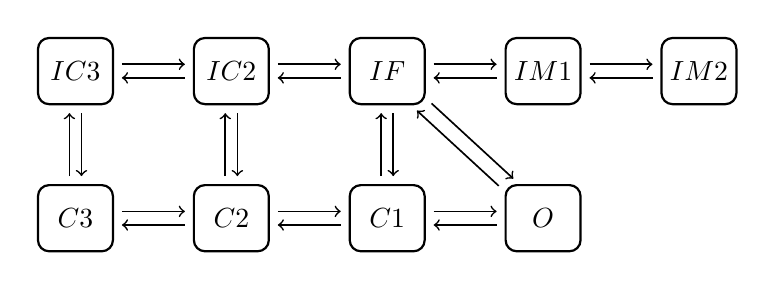
\begin{tikzpicture}[
   font=\sffamily,
   every matrix/.style={ampersand replacement=\&,column sep=1cm,row sep=1cm},
   state/.style={draw,thick,rounded corners,inner sep=.3cm},
   to/.style={->,semithick,shorten >=0.1cm,shorten <=0.1cm},
   Q/.style={->,semithick,sloped,pos=0.700000,shorten >=0.1cm,shorten <=0.1cm},
   every node/.style={auto}]
\matrix{
\node[state] (IC3) {\parbox{10pt}{\centerline{$IC3$}}};\&\node[state] (IC2) {\parbox{10pt}{\centerline{$IC2$}}};\&\node[state] (IF) {\parbox{10pt}{\centerline{$IF$}}};\&\node[state] (IM1) {\parbox{10pt}{\centerline{$IM1$}}};\&\node[state] (IM2) {\parbox{10pt}{\centerline{$IM2$}}};\\
\node[state] (C3) {\parbox{10pt}{\centerline{$C3$}}};\&\node[state] (C2) {\parbox{10pt}{\centerline{$C2$}}};\&\node[state] (C1) {\parbox{10pt}{\centerline{$C1$}}};\&\node[state] (O) {\parbox{10pt}{\centerline{$O$}}};\&\\
};
\draw[to]  (IC3.10) to node {$$} (IC2.170);
\draw[to]  (IC3.280) to node {$$} (C3.80);
\draw[to]  (IC2.190) to node {$$} (IC3.350);
\draw[to]  (IC2.10) to node {$$} (IF.170);
\draw[to]  (IC2.280) to node {$$} (C2.80);
\draw[to]  (IF.190) to node {$$} (IC2.350);
\draw[to]  (IF.10) to node {$$} (IM1.170);
\draw[to]  (IF.280) to node {$$} (C1.80);
\draw[Q]  (IF.325) to node {$$} (O.125);
\draw[to]  (IM1.190) to node {$$} (IF.350);
\draw[to]  (IM1.10) to node {$$} (IM2.170);
\draw[to]  (IM2.190) to node {$$} (IM1.350);
\draw[to]  (C3.100) to node {$$} (IC3.260);
\draw[to]  (C3.10) to node {$$} (C2.170);
\draw[to]  (C2.100) to node {$$} (IC2.260);
\draw[to]  (C2.190) to node {$$} (C3.350);
\draw[to]  (C2.10) to node {$$} (C1.170);
\draw[to]  (C1.100) to node {$$} (IF.260);
\draw[to]  (C1.190) to node {$$} (C2.350);
\draw[to]  (C1.10) to node {$$} (O.170);
\draw[Q]  (O.145) to node {$$} (IF.305);
\draw[to]  (O.190) to node {$$} (C1.350);
\end{tikzpicture}
\end{center}
\caption{The sodium channel model of Clancy et al. \cite{Clancy2002}\label{clancy}; O is the open state, C1, C2 and C3 are the closed states, while the rest of the states represent different kinds of inactivation.}
\end{figure}
%{\it Glenn: forklar hva IM1, IM2 osv betyr i dette skjemaet.}

The popularity of these models stems from the fact that it is possible to adjust the parameters involved to obtain a model that reflects data quite well. However, it should also be mentioned that models can be so complex that it is virtually impossible to uniquely determine all the parameters involved. In these notes, we shall confine ourselves to relatively simple Markov models but the methods we describe can be applied, at least in principle, to Markov models of higher complexity.


\subsection{The master equation}
\label{master_equation}

From the Markov model written on the form (\ref{Markov1}), we can derive an equation
giving the evolution of the probability of the two states, open (O) and closed (C). Let $o=o(t)$ be the
probability that the channel is in the open (O) state at time $t$ and let $c=c(t)$ denote
the probability that the channel is closed (C). We assume that the probabilities $o$ and $c$ are known at time
$t$ and then use the Markov model (\ref{Markov1}) to compute the probabilities at time $t+\Delta t$.
 Here $\Delta t$ is assumed to be so small that the channel changes state at most once during the time step from $t$ to $t+\Delta t$.   Then the scheme (\ref{Markov1}) states that
the open probability at time $t+\Delta t$ is given by
\begin{align}
o(t+\Delta t) &= \text{Prob}\left[  (S(t)=C)  \mbox{\ and\ }  (C\rightarrow O \mbox{\ during\ } \Delta t)  \right] \\
& \ \ \ \ + \text{Prob}\left[  (S(t)=O)  \mbox{\ and not}  (O\rightarrow C \mbox{\ during\ } \Delta t)  \right] \\
&= c(t) \cdot (\Delta t k_{co}) + o(t) \cdot (1 -\Delta t k_{oc})
\end{align}
so
\[
o(t+\Delta t)=o(t)+\Delta t ( k_{co}c(t)-k_{oc}o(t)).
\]
%which expresses the fact that, during the time step from $t$ to $t+\Delta t$, the channel either remain open (first term), it changes from open to close (second term) or it changes from closed to open (last term).
From this equation, we obtain
\[
\frac{o(t+\Delta t)-o(t)}{\Delta t}=k_{co}c(t)-k_{oc}o(t),
\]
and, therefore, by passing to the limit $\Delta t\rightarrow0,$ we get the
differential equation
\begin{equation}
o^{\prime}(t)=k_{co}c(t)-k_{oc}o(t).\label{po}
\end{equation}
Similarly, we find that the probability of being in the closed state evolves
according to
\begin{equation}
c^{\prime}(t)=k_{oc}o(t)-k_{co}c(t).\label{pc}
\end{equation}
Since we are dealing with probabilities, it is reasonable to assume that the
initial conditions add up to one (the channel is either open or closed) and therefore, by adding the equations
above, we find that
\[
o(t)+c(t)=1
\]
for all time. Hence the variable $c$ in (ref{po}) can be
replaced by $1-o$ and the system (ref{po},\ref{pc}) can be
written as a scalar equation of the form
\begin{equation}
o^{\prime}(t)=\left(  k_{co}+k_{oc}\right)  \left(  \frac{k_{co}}
{k_{co}+k_{oc}}-o\left(  t\right)  \right)  .\label{po2}
\end{equation}
Here we see that
\[
o=\frac{k_{co}}{k_{co}+k_{oc}}
\]
is a stable equilibrium solution. Furthermore, if we know that the channel is
closed initially, that is, $o(0)=0,$ we get the solution
\[
o(t)=\frac{k_{co}}{k_{co}+k_{oc}}\left(  1-e^{-\left(  k_{co}+k_{oc}\right)
t}\right)
\]
and we notice that the equilibrium is reached more quickly as the sum of the rates
$k_{co}+k_{oc}$ increases.

\subsection[Three state model]{The master equation of a three-state model}

The development of the master equation for the two-state model above can be
carried out for any Markov model. For instance, if we consider the three-state
Markov model shown in Figure \ref{IOC_me}, we realize that the probabilities of the
open (O), closed (C), and inactivated (I) states are governed by the following system of ordinary
differential equations:
\begin{align}
o^{\prime}  & =k_{io}i+k_{co}c-\left(  k_{oi}+k_{oc}\right)  o, \nonumber \\
c^{\prime}  & =k_{oc}o+k_{ic}i-\left(  k_{co}+k_{ci}\right)  c,\label{me_11}\\
i^{\prime}  & =k_{oi}o+k_{ci}c-\left(  k_{io}+k_{ic}\right)  i, \nonumber
\end{align}
Since
\begin{equation}
i=1-\left(  o+c\right),
\end{equation}
we have the following $2 \times 2$ system:
\begin{align}
o^{\prime}  & =k_{io}+\left(  k_{co}-k_{io}\right)  c-\left(  k_{oi}
+k_{oc}+k_{io}\right)  o,\label{me_20}\\
c^{\prime}  & =k_{ic}+\left(  k_{oc}-k_{ic}\right)  o-\left(  k_{co}
+k_{ci}+k_{ic}\right)  c.\label{me_21}
\end{align}
We will now show, using a numerical computation, that the solution of the
system (\ref{me_20},\ref{me_21}) coincides with the average result of Monte Carlo simulations using
the Markov model shown in Figure \ref{IOC_me} as the number of Monte Carlo runs goes
to infinity.



\begin{figure}[ptb]
\begin{center}
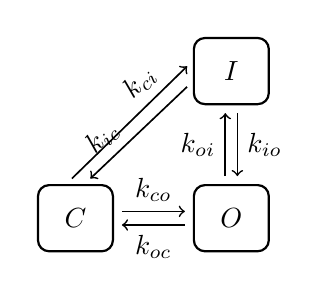
\begin{tikzpicture}[
   font=\sffamily,
   every matrix/.style={ampersand replacement=\&,column sep=1cm,row sep=1cm},
   state/.style={draw,thick,rounded corners,inner sep=.3cm},
   to/.style={->,semithick,shorten >=0.1cm,shorten <=0.1cm},
   Q/.style={->,semithick,sloped,pos=0.700000,shorten >=0.1cm,shorten <=0.1cm},
   every node/.style={auto}]
\matrix{
\&\node[state] (I) {\parbox{10pt}{\centerline{$I$}}};\\
\node[state] (C) {\parbox{10pt}{\centerline{$C$}}};\&\node[state] (O) {\parbox{10pt}{\centerline{$O$}}};\\
};
\draw[to]  (O.100) to node {$k_{oi}$} (I.260);
\draw[to]  (O.190) to node {$k_{oc}$} (C.350);
\draw[to]  (I.280) to node {$k_{io}$} (O.80);
\draw[Q]  (I.195) to node {$k_{ic}$} (C.75);
\draw[to]  (C.10) to node {$k_{co}$} (O.170);
\draw[Q]  (C.105) to node {$k_{ci}$} (I.165);
\end{tikzpicture}
\end{center}
\caption{Markov model including three possible states: open (O), closed (C), and
inactivated (I).}
\label{IOC_me}
\end{figure}




\subsection[Monte Carlo Simulations]{Monte Carlo simulations based on the Markov model}
\label{MCSMM}

Before we compare the two computational schemes, let us briefly describe how
the Monte Carlo simulation can be implemented. We choose a small timestep
$\Delta t$ and we assume that the state at time $t=t_{n}=n\Delta t,$ where $n$
is a non-negative integer, is either O, C, or I. For simplicity, we describe how
the computation proceeds in the case of the channel being in the open (O)
state at time $t=t_{n}$. In order to decide the state at time $t_{n+1}=t_{n}+\Delta t,$ we
divide the unit interval into three non-overlapping parts:  $A_{c}=\left[
0,k_{oc}\Delta t\right)  ,$ $A_{i}=\left[  k_{oc}\Delta t,k_{oc}\Delta
t+k_{oi}\Delta t\right)  ,$ $A_{o}=\left[  k_{oc}\Delta t+k_{oi}\Delta
t,1\right]  .$ Then, at time $t_{n+1}=t_{n}+\Delta t,$ we can update the state
of the channel based on a random number $r_{n}$ in the unit interval drawn from
a uniform distribution. Specifically, if $r_{n}\in A_{o},$ the channel
remains open; if $r_{n}\in A_{c},$ the state of the channel changes from
open to closed; and, finally, if $r_{n}\in A_{i},$ the state of the channel
changes from open to inactivated.

Similar steps are straightforward to
devise for the case of the channel being in the closed or inactivated states
at time $t=t_{n}.$



\subsection[Monte Carlo simulation vs Master Equation]{Comparison of Monte Carlo simulations and solutions of the
master equation}

In Figure \ref{Introduction_L:ode_mc} we compare the probabilities computed by solving the master equation (ref{me_20},\ref{me_21}) (red lines) and by Monte Carlo simulations using the Markov model as described above. In the simulations we have used the initial conditions $o(0)=i(0)=0$
and $c(0)=1$ and the rates used in the computations are given in Table \ref{tab:const3x3}. As the number of Monte Carlo simulations increases, we see that the average approaches the solution of the continuous master equation. In these computations the master equation was solved using the function \GTLV{ODE15s in Matlab}.


\begin{table}  \begin{center}
\begin{tabular}{|r|r|r|r|r|r|} \hline
$k_{oi}$ & $k_{io}$ & $k_{co}$ & $k_{oc}$ & $k_{ic}$ &$k_{ci}$  \\ \hline
0.5  &    0.3 &   0.6   &  0.9  &   0.72  & 0.8 \\ \hline
\end{tabular} \end{center}
\caption{Rates (in 1/ms) of the Markov model given in Figure  \ref{IOC_me} used in the computations presented in Figure \ref{Introduction_L:ode_mc}.}
 \label{tab:const3x3}  \end{table}


%xxGlenn: Lag gjerne 3x3 paneler, der o,c,og i g\aa r fra venstre mot h\o yre og der antall MC \o ker (og dt reduseres) ovenfra og ned. Alle detaljer i caption og i tabellene nevnt over.

FIGURE: [fig/Introduction_L_ode_mc.pdf, width=500 frac=0.8]  Comparison of the solution of the master equation (ref{me_20},\ref{me_21}) (red lines) and the results of Monte Carlo simulations based on the Markov model given in Figure \ref{IOC_me}. The time step used in the Monte-Carlo simulations was $\Delta t$ = 0.01 ms in all the panels and the simulations were run for 10 ms. The number of Monte Carlo simulations increases from 100 (top) to 10,000 (bottom). label{Introduction_L:ode_mc}


\subsection{Equilibrium probabilities}
\label{eq_prob_ioc}

The equilibrium state of the
reaction shown in Figure  \ref{IOC_me} is characterized by the equations
\begin{align}
k_{co}c  &  =k_{oc}o, \nonumber\\
k_{oi}o  &  =k_{io}i, \label{me_eq_20}\\
k_{ic}i  &  =k_{ci}c, \nonumber
\end{align}
where $o,c,$ and $i$ denote the probabilities of the channel being open,
closed, or inactivated, respectively. It follows that
\[
c=\frac{k_{oc}}{k_{co}}o
\]
and
\[
i=\frac{k_{oi}}{k_{io}}o.
\]
By using the fact that $o+c+i=1,$ we obtain
\[
\left(  1+\frac{k_{oc}}{k_{co}}+\frac{k_{oi}}{k_{io}}\right)  o=1
\]
and therefore
\begin{align*}
o  &  =\frac{1}{1+\frac{k_{oc}}{k_{co}}+\frac{k_{oi}}{k_{io}}},\\
c  &  =\frac{\frac{k_{oc}}{k_{co}}}{1+\frac{k_{oc}}{k_{co}}+\frac{k_{oi}
}{k_{io}}},\\
i  &  =\frac{\frac{k_{oi}}{k_{io}}}{1+\frac{k_{oc}}{k_{co}}+\frac{k_{oi}
}{k_{io}}}.
\end{align*}
For the particular rates given in Table \ref{tab:const3x3}, we get the following equilibrium probabilities: $o=0.24,\, c=0.36$, and
$i=0.4$.

\subsection{Detailed balance}

In order to compute the equilibrium solution of (\ref{me_11}) above, we assumed that each of the sub-transitions of the diagram given in Figure \ref{IOC_me} was in equilibrium. More precisely, we assumed that
\[k_{co}c    =k_{oc}o, \, k_{oi}o =k_{io}i,  \text{ and }k_{ic}i =k_{ci}c. \]
These three relations yield
\begin{equation}
k_{co}k_{oi}k_{ic}=k_{ci}k_{io}k_{oc}. \label {db}
\end{equation}
This relation is referred to as the condition of {\it detailed balance}. In these notes, we will always assume that Markov models satisfy this condition. More generally, the product of the rates in a loop (e.g. the I-O-C loop of Figure \ref{IOC_me}) in the clockwise direction equals the product of the rates in the counterclockwise direction. Under this assumption, the equilibrium solution can always be computed by the method indicated above. We will use the same technique many times in these notes.



\section{The master equation and the equilibrium solution}
\label{me_eq}

We have seen that the Markov model written in the form
\begin{equation}
C\underset{k_{co}}{\overset{k_{oc}}{\leftrightarrows}}O \label{Markov1010}
\end{equation}
leads to a master equation of the form
\begin{align}
o^{\prime}(t)=  &  k_{co}c(t)-k_{oc}o(t),\label{po1010}\\
c^{\prime}(t)=  &  k_{oc}o(t)-k_{co}c(t). \label{pc1010}
\end{align}
Since $o+c=1,$ we can reduce the system to the scalar equation,
\[
o^{\prime}(t)=\left(  k_{co}+k_{oc}\right)  \left(  \frac{k_{co}}
{k_{co}+k_{oc}}-o\left(  t\right)  \right)
\]
and we readily see that the equilibrium solution is given by
\[
o=\frac{k_{co}}{k_{co}+k_{oc}}.
\]
Exactly the same steps can be followed for the three-state Markov model
illustrated in Figure \ref{IOC_me}. The associated Markov model reads
\begin{align*}
o^{\prime} &  =k_{io}i+k_{co}c-\left(  k_{oi}+k_{oc}\right)  o\\
c^{\prime} &  =k_{oc}o+k_{ic}i-\left(  k_{co}+k_{ci}\right)  c\\
i^{\prime} &  =k_{oi}o+k_{ci}c-\left(  k_{io}+k_{ic}\right)  i
\end{align*}
and since
\begin{equation}
i=1-\left(  o+c\right)  \label{i4010}
\end{equation}
we arrive at the following $2 \times 2$ system:
\begin{align*}
o^{\prime} &  =k_{io}+\left(  k_{co}-k_{io}\right)  c-\left(  k_{oi}
+k_{oc}+k_{io}\right)  o,\\
c^{\prime} &  =k_{ic}+\left(  k_{oc}-k_{ic}\right)  o-\left(  k_{co}
+k_{ci}+k_{ic}\right)  c.
\end{align*}
The equilibrium solution is now defined by a $2 \times 2$ linear system of equations of
the form
\begin{equation}
Bq=b,\label{i4011}
\end{equation}
where
\[
B=\left(
\begin{array}
[c]{cc}
k_{oi}+k_{oc}+k_{io} & k_{io}-k_{co}\\
k_{ic}-k_{oc} & k_{co}+k_{ci}+k_{ic}
\end{array}
\right)  ,\;q=\left(
\begin{array}
[c]{c}
o\\
c
\end{array}
\right)  \text{, and }b=\left(
\begin{array}
[c]{c}
k_{io}\\
k_{ic}
\end{array}
\right)  .\;
\]
By solving this linear system and using (ref{i4010}), we
find (as above) that

\[
o=K^{-1},\;c=\;\frac{k_{oc}}{k_{co}}K^{-1},\;i=\frac{k_{oi}}{k_{io}}K^{-1},
\]
where
\[
K=1+\frac{k_{oc}}{k_{co}}+\frac{k_{oi}}{k_{io}}.
\]

\subsection[Linear algebra]{Linear algebra approach to finding the equilibrium solution}

Calculations to find the equilibrium solution will be done repeatedly in these notes. We
will always use the special structure of the Markov model to derive the
equilibrium solution, but it also worth noting that this can be done by
solving a linear system. The master equation associated with a Markov model of the
form  (ref{Markov1010}) or of the form given in
Figure \ref{clancy} can always be written in the form
\[
p^{\prime}=Ap,
\]
where $p$ is a vector containing the probabilities of occupying the different
states of the Markov model. Since the sum of the probabilities adds up to one,
the number of unknowns can be reduced by one and the system takes the form
\[
q^{\prime}=b-Bq.
\]
Therefore, the equilibrium solution can be found by solving the linear system
(ref{i4011})

Instead of reducing the number of unknowns, we can also address the problem more directly by computing the eigenvector
associated the eigenvalue $\lambda = 0$. For instance, using Matlab  we can put $z=\rm{null}(A)$ and then define
\[p=\frac{z}{\sum_i z_i}\]
 where
$z_i$ denote the components of the vector $z$.


\section[Stochastic simulations and PDFs]{Stochastic simulations and probability density functions}

Given the Markov model, defining a stochastic differential equation describing changes of the transmembrane potential due to the opening and closing of the channel is quite straightforward. Additionally, based on the stochastic differential equation, we will derive deterministic differential equations describing the probability density functions of the states involved in the Markov model. We thus have two ways to analyze models of ion channels: We can either run numerous Monte Carlo simulations using the stochastic differential equation or solve the deterministic differential equations defining the probability density functions. Both these methods will be used throughout the notes. Although one method is the average of the other, we will see that both provide distinct insights useful to understanding the mechanisms under consideration.


\section{Markov models of calcium release}
The contraction of the heart is a collective and very well-coordinated effort achieved in a collaboration involving billions of cells. For each of these cells, the contraction depends on the release of a massive amount of calcium from internal storage. The release takes place in many thousands of release units within each cell and the state of the release process is believed to be adequately modeled using Markov models.

We will study this release in several steps and we start by assuming that the only varying concentration is in the dyad and that the reaction rates of the Markov model vary only with this single concentration. This case will be studied in great detail and we will explain how drugs can be theoretically constructed to repair mutations affecting the release mechanism. The analysis is based on a scalar stochastic differential equation representing the concentration of calcium in the dyad. The properties of this model will be analyzed using Monte Carlo simulations. Furthermore, we will derive a system of deterministic partial differential equations describing the probability density function of the states of the Markov model.

It is more common to divide the calcium concentration into two values---not only one---which leads to  $2\times2$ stochastic differential equations to be analyzed. This model will also be analyzed using Monte Carlo simulations and by a 2D deterministic system of partial differential equations representing the probability density functions of the states of the Markov model.

Next, we shall couple the calcium concentration to the voltage-gated release of calcium through so-called L-type calcium channels. This model will allow us to study optimal drugs, combining the effect on calcium release and L-type channels. The balance of these mechanisms rules the calcium-induced calcium release that is at the crux of cardiac contraction. The calcium-induced calcium release model is stated in terms of a $2\times 2$ model of stochastic equations where the transmembrane potential $V$ is included as a parameter in the model. The associated model for the probability density functions is given by a 2D system of partial differential equations where the transmembrane potential is again included as a parameter.

 \section{Markov models of ion channels}

After analysis of the calcium release we move on to study voltage-gated  ion channels. We will immediately see that in mathematical terms the problem is very similar to the calcium release problem. For the ion channel case, however, the stochastic equation is one-dimensional and so is the associated deterministic partial differential equation. The basic Markov model is still based on the open and closed states, but we will also see that an inactivated state plays a central role. Optimal theoretical drugs will be derived and we will observe that they work nicely.

\section{Mutations described by Markov models}

A trademark of mutations affecting ion channels and calcium release mechanisms is that they change the open probability and possibly also the mean open time and other characteristics of the channels involved. We will show below that the equilibrium open probability of the channel described by the Markov model of the form (\ref{Markov1}) is given by
\[ o=\frac{k_{co}}{k_{co}+k_{oc}} \]
and the mean open time is given by
\[ \tau_o=\frac{1}{k_{oc}}. \]
The concept of mean open time will be discussed in Chapter \ref{mot_chapter} and the formula $\tau_o=1/k_{oc}$ will be derived in that chapter.
 Given these formulas, it is straightforward to see that the effect of mutations affecting the open probability or the mean open time can be modeled by changing the parameters of the Markov model. In these notes we shall focus on rather simple changes
 in the model but, again, the techniques can be generalized to more intricate cases.

  Two examples of the effect of mutations are given in Figures
 \ref{Introduction_L:Loaiza_crop}  and \ref{Introduction_L:chandra}. Figure
 \ref{Introduction_L:Loaiza_crop}  shows recordings of the open and closed states for the wild type and the
  V2475F mutation of the ryanodine receptor (RyR).
  The graphs in Figure \ref{Introduction_L:chandra} show similar results for the voltage-gated sodium channel when the wild type recordings are compared with recordings from a mutant ($\Delta$KPQ) channel.


FIGURE: [fig/Introduction_L_Loaiza_crop.png, width=500 frac=0.8] Single-channel recordings of wild type (black) and mutant (red) cardiac RyR channels. The open probability and the mean open time are significantly increased for the mutant (V2475F) case. The graphs are from Figure 3 of Loaiza et al. \cite{loaiza2013}. label{Introduction_L:Loaiza_crop}

FIGURE: [fig/Introduction_L_chandra.png, width=500 frac=0.8] Sodium current recordings taken from Figure 4 of Chandra et al. \cite{Chandra1998}: A represents the wild type and B represents
the $\Delta$KPQ mutant. The recordings are based on 200-ms depolarizing pulses from -100 mV to -40 mV.  label{Introduction_L:chandra}


\section{The problem and steps toward solutions}

Assume that experimental data on wild type cells can be used to identify the parameters of a Markov model faithfully describing the stochastic properties of the wild type channel and that experimental data on mutant cells can be used to establish a Markov model of similar structure representing the stochastic properties of the mutant channel. Furthermore, we assume that the Markov model of the mutant can be extended to account for the effect of a theoretical drug. {\it The problem is then to compute the reaction rates of the drug such that, after the drug is applied, the mutant channel behaves as similarly to the wild type channel as possible. } The essence of these notes is to show how to solve this problem mathematically; we show how to compute an optimal theoretical drug. To clarify what we mean by an optimal theoretical drug, we will give a few examples that will be discussed later and then we will briefly discuss the concept of a theoretical drug  more generally.

 \subsection{Markov models for drugs: Open state and closed state blockers}
 By using the notation of chemical reactions introduced above, we can explain the problem in a bit more detail. The reaction scheme for an open state blocker can be illustrated as follows:
\begin{equation}
C\underset{ k_{co}}{\overset{k_{oc}}{\leftrightarrows}}O\underset{k_{ob}
}{\overset{k_{bo}}{\leftrightarrows}}B. \label{open_block}
\end{equation}
For theoretical purposes, this drug is well defined, provided that we know the values of the parameters $k_{ob}$ and $k_{bo}$. We will often assume that these parameters are constants. As mentioned above, one example of a problem we want to overcome
is mutations leading to an increased open probability; so either the release mechanism is too prone to releasing calcium from internal storage or the ion channels are too prone to allowing  current to flow through the cell membrane.

Since the problem involves too high of an open probability, it seems reasonable to try to fix the open probability by extending the reaction scheme and directly affecting this state, as illustrated in the reaction scheme above. By allowing the probability to be moved from $O$ to $B$, the open probability will be reduced and thus the goal will be achieved. This reasoning seems impeccable and it seems much less intuitive to use a closed state drug of the form
\begin{equation}
B\underset{k_{bc}}{\overset{k_{cb}}{\leftrightarrows}}C\underset{
k_{co}}{\overset{k_{oc}}{\leftrightarrows}}O. \label{closed_block}
\end{equation}
We will see, however, that both open and closed state blockers may be optimal, depending on the nature of the mutation.

\subsection{Closed to open mutations (CO-mutations)}
\label{com}
We have seen that for a Markov model written in the form
\begin{equation}
C\underset{ k_{co}}{\overset{k_{oc}}{\leftrightarrows}}O,
\end{equation}
 the equilibrium open probability is given by
\[ o=\frac{k_{co}}{k_{co}+k_{oc}}=\frac{1}{1+\frac{k_{oc}}{k_{co}}} \]
and the mean open time is given by
\[ \tau_o=\frac{1}{k_{oc}}. \]
A mutation leading to an increased open probability can be represented by a Markov model written in the form
\begin{equation}
C\underset{ \mu k_{co}}{\overset{k_{oc}}{\leftrightarrows}}O,
\end{equation}
where $\mu \ge 1$ will be referred to as the {\it mutation severity index} and we always use the convention that $\mu=1$ refers to the wild type case. At this point, it is useful to recall the interpretation of a scheme of this form. In particular, it is useful to note that the probability of going from the closed state (C) to the open state (O) during a time step $\Delta t$ is now given
by $\mu \Delta t k_{co}$, compared to $\Delta t k_{co}$ for the wild type channel. It is pretty clear that increasing the mutation severity index will increase the probability of being in the open state and this is also reflected by the equilibrium open probability given by
\[o_\mu=\frac{1}{1+\frac{k_{oc}}{\mu k_{co}}}, \]
which clearly increases as a function of the mutation severity index $\mu$.
It is also interesting to observe that, for this mutation, the mean open time is unchanged. We will refer to a mutation of this form as a CO-mutation and we will show repeatedly that, for CO-mutations, closed state blockers are theoretically optimal.

\subsection{Open to closed mutations (OC-mutations)}
Another way to introduce a mutation that increases the open probability is to decrease the rate from open to closed. This can be written as follows:
\begin{equation}
C\underset{ k_{co}}{\overset{k_{oc}/\mu}{\leftrightarrows}}O,
\end{equation}
where, again, $\mu \ge 1$ is the mutation severity index and $\mu=1$ represents the wild type. The probability of leaving the open state is now reduced and this will lead to an increased open probability.
In particular, the equilibrium open probability is again given by
\[ o_\mu=\frac{1}{1+\frac{k_{oc}}{\mu k_{co}}}, \]
as above, but now the mean open time changes; it is given by
\[ \tau_o=\frac{\mu}{k_{oc}}\]
and thus increases with the mutation severity index.

We will refer to a mutation of this form as an OC-mutation and we will show that, for such mutations, open state blockers are theoretically optimal.

\section{Theoretical drugs}
\label{theoreticaldrugs}

The concept of a theoretical drug is essential in these notes. Basically, we will {\em  refer to a theoretical drug\footnote{We also use the terms \textit{mathematical drug, numerical drug}, and so forth interchangeably with \textit{theoretical drug}} as a purely mathematical construction} that may or may not have a viable pharmaceutical counterpart. A mental image of how the drug may work is given in Figure \ref{Introduction_L:drg_starmer}; the figure is taken from Starmer \cite{Starmer2002}. With no drug involved, the channel can take on two conformational states: the open state (O), when ions can flow freely through the channel, and the closed state (C), when there is no flow of ions through the channel. An open blocker can change the open state such that there is no flow through the channel. The reaction scheme of the situation described in the figure is given by
\begin{equation}
C\underset{ k_{co}}{\overset{k_{oc}}{\leftrightarrows}}O\underset{k_{ob}
}{\overset{k_{bo}}{\leftrightarrows}}B. \label{closed_block201}
\end{equation} where we again note that the properties of the theoretical drug are solely given by the values of the rates $k_{ob}$ and $k_{bo}$.

This way of describing the effect of a drug has been used for many years, see e.g. Hille \cite{Hille1977} or Hondeghem and Katzung \cite{Hondeghem1977}. Our use of this notation is clearly motivated by the paper of Clancy et al. \cite{Clancy2007}. In these papers, an existing drug is characterized using a scheme of the form (\ref{closed_block201}). That is, data obtained from experiments using a particular drug are used to characterize the rates $k_{bo}$ and $k_{ob}$ referred to, respectively, as the on and off rates of the drug. As mentioned above, we often view the rates as free parameters that can be optimized in order to create the best possible theoretical drug in the sense that the channel should work as much like the healthy case as possible. This way of describing a theoretically optimal drug was introduced in \cite{Tveito2011c} and clearly motivated by the drug vector approach discussed in   \cite{Tveito2009}.

FIGURE: [fig/Introduction_L_drg_starmer.png, width=500 frac=0.8] Illustration of a blocker associated with the open state. In the leftmost case the channel is closed and no ions can pass through it. In the center case, the channel is open and ions may flow freely. In the rightmost case the channel is blocked by the drug and no ions can pass through it. The figure is taken from Starmer \cite{Starmer2002}. label{Introduction_L:drg_starmer}

\section{Results}
Many of the models, methods, and results described in these notes are well known in the literature. All the Markov models are taken from the literature and so are the stochastic differential equations and the models describing the probability density approach. Compared to earlier published models, we will often derive simplified models, but the ideas behind them are basically the same as those used by many authors. Concerning the modeling of mutations, we aim to consistently model the effect of mutations as simply as possible and preferably only by changing a single parameter: the mutation severity index.

The novel part of these notes is that we attempt to systematically describe how to compute characterizations of drugs that are optimal in a specific sense and we do so for a number of applications. We almost exclusively address so-called gain-of-function mutations. For such mutations, the open probability of the channel or receptor is too large, which can lead to severe difficulties for the cell and, ultimately, for large collections of such cells.

%We begin by studying such mutations in cases where the mean open time is unaltered. In such cases, we give several examples indicating that closed blockers are much better suited for repairing the effect of the mutation than open blockers. If, on the other hand, both the open probability and the mean open time is affected, open state blockers are to be preferred. In a similar manner we discuss how to deal with mutations that impair the inactivation of ion channels.

\section{Other possible applications}

The focus in this text will be on how to compute characterizations of optimal theoretical drugs defined in terms of parameters describing the associated Markov model. The methods can, however, also be used to compare existing drugs. If Markov models are developed for two drugs, the associated probability density functions can be computed and thus a comparison of the quality of the two drugs can be computed. This approach will rely heavily on accurate representations of the function of a drug in terms of a Markov model, which is a problem beyond the scope of the present notes.


\section{Disclaimer}
These notes are written to explain in some detail how we can compute characterizations of theoretical drugs in terms of Markov models. However, we specifically avoid discussing whether it is possible to realize a certain drug given the characterization in terms of a Markov model, simply because we do not know and have been unable to find any reasonable answer to this in the literature.  The applicability of our results therefore remains uncertain.


\section{Notes}
\begin{enumerate}
\item Several excellent introductions to Markov models of the stochastic behavior of receptors and ion channels are available (e.g., \cite{KeenerSneyd, Smith2002, Jacobs2010, Santillan2014}). In particular we recommend the recently published book by Bressloff \cite{Bressloff2014} (see also \cite{Bressloff2014w}). Bressloff \cite{Bressloff2014} provides a broad introduction to stochastic processes in cells and covers most of the models covered in the present text and much more. It is an excellent text that will become a standard reference in the field.
\item A comprehensive mathematical analysis of the stochastic properties of single ion channels using Markov models was initiated by Colquhoun and Hawkes (e.g., \cite{ Colquhoun1977,Colquhoun1981,Colquhoun1982}).
\item Insight into the electrophysiology of excitable cells was fundamentally enhanced by the development of the patch clamp technique of Sakmann and Neher (see, e.g., \cite{Sakmann1984,Sakmann1995}). The authors received the Nobel Prize in Physiology or Medicine in 1991 for their work on single ion channels. The patch clamp technique is used to generate measurements of the form illustrated in
Figure \ref{Introduction:na_cropped}. These data are used to determine the Markov model and are therefore of fundamental importance. As mentioned below, however, the problem of finding the Markov model based on experimental data is still an active research problem.
\item The models studied in these notes address the flow of ions through various types of channels. An excellent introduction to ion channels is given in the book by Hille \cite{Hille2001}.
\item Our discussion is focused on mechanisms of the heart but, at the level of single channels, these mechanisms are similar to channel-based mechanisms of the brain or, more specifically, the mechanisms of neurons. There are several excellent introductions to neuroscience
(e.g., \cite{Ermentrout2010,Sterratt2011,Dayan2001,Izhikevich2007}).
\item
Given the Markov model, we have seen that it is pretty straightforward to compute what state the channel is in as a stochastic function of time. We have also seen that we can solve the master equation and find the average behavior of the channel when the rates are independent of the surroundings. Furthermore, we will show how to compute probability density functions for each state when the rates depend on the transmembrane potential. Such simulations are forward problems: Given the model,  compute the solution. The inverse problem in this setting is quite a bit harder; the problem is to compute the rates (i.e., the values of $k_{oc},\,  k_{co}$ etc.) of the Markov model in order for the stochastic behavior of the model to match the measurements of the channel. The analysis of the inverse problem was started by Colquhoun and Hawkes \cite{Colquhoun1977}, beginning in 1977, and their findings are summarized by Sakmann and Neher \cite{Sakmann1995} (see also
\cite{Colquhoun1996}). More recently the problem has been addressed in a series of papers by Sachs and his co-authors; see \cite{Qin1996,Qin2000,Nicolai2013}. Their methods are available in the open-source QuB software package. Furthermore, Markov chain Monte Carlo (MCMC) has been used in a series of papers by Siekmann, Sneyd and his co-authors \cite{Gin2009,Siekmann2011,Siekmann2012, Siekmann2014}. Interestingly, their analysis shows that certain Markov models cannot be identified using standard data. The MCMC method was used for inversion of single ion channel data more than 15 years ago by Ball et al \cite{Ball1999}, and Rosales and co-authors, see \cite{Rosales2001,Rosales2004}.
\item For whole cell data, the problem of identifying the parameters of Markov models is carefully studied by Fink and Noble \cite{Fink2009}.
\item The terms {\it CO-mutation}, {\it OC-mutation}, and {\it mutation severity index} are not standard and introduced here for convenience.
\item A thorough discussion of the principle of detailed balance can be found in the paper by  Colquhoun et al. \cite{Colquhoun2004}. The validity of the principle for given data can be tested as shown by Song and Magleby \cite{Song1994} and Ullah et al. \cite{Ullah2012} (suppl. material).
There are examples of Markov models that do not satisfy the principle of detailed balance (see, e.g., \cite{Bressloff2014}, p. 208).
\item The numerical method for handling the Markov model described on page \pageref{MCSMM} is not particularly efficient. For the case of constant rates in the Markov model, considerable acceleration can be achieved by using the method of Gillespie \cite{Gillespie1977}. The Gillespie method is particularly useful for simulations involving many channels (see, e.g., \cite{Smith2002}).
\item For comprehensive introductions to modeling the cardiac action potential, we refer to the recent overview by Rudy \cite{Rudy2012} and to Rudy and Silva \cite{Rudy2006}.  For the action potential shown in Figure \ref{Introduction_L:grandi}, we used the model of Grandi et al. \cite{Grandi2010B}. An alternative is the model of O'Hara et al. \cite{Ohara2011} and a huge collection of models is available at the CellML project (CellML.org).
\item The dynamics of cardiac electrophysiology are introduced in numerous papers and books; a recent comprehensive review is provided by Qu et al. \cite{Qu2014}.  The book by Katz \cite{Katz2010}
is a standard reference in cardiac physiology and the book by Glass et al. \cite{Glass2012} is a standard reference in the modeling of the heart. Numerical methods for the simulation of cardiac electrophysiology are presented by Sundnes et al. \cite{Sundnes2007} (see also \cite{Pullan2005, Franzone2014}).



\end{enumerate}









